\documentclass[a4paper,11pt]{article}
\usepackage[T1]{fontenc}
\usepackage[utf8]{inputenc}
\usepackage{lmodern}
\usepackage{hyperref}
\usepackage{graphicx}
\usepackage{rotating}
\usepackage{listings}
\usepackage{color}
\usepackage{listings}
\usepackage{pdfpages}

\title{Advanced Algorithms - part 2 (exc 4-6) by}
\author{Arash Rouhani (rarash@student.chalmers.se) - 901117-1213}


\begin{document}

\maketitle

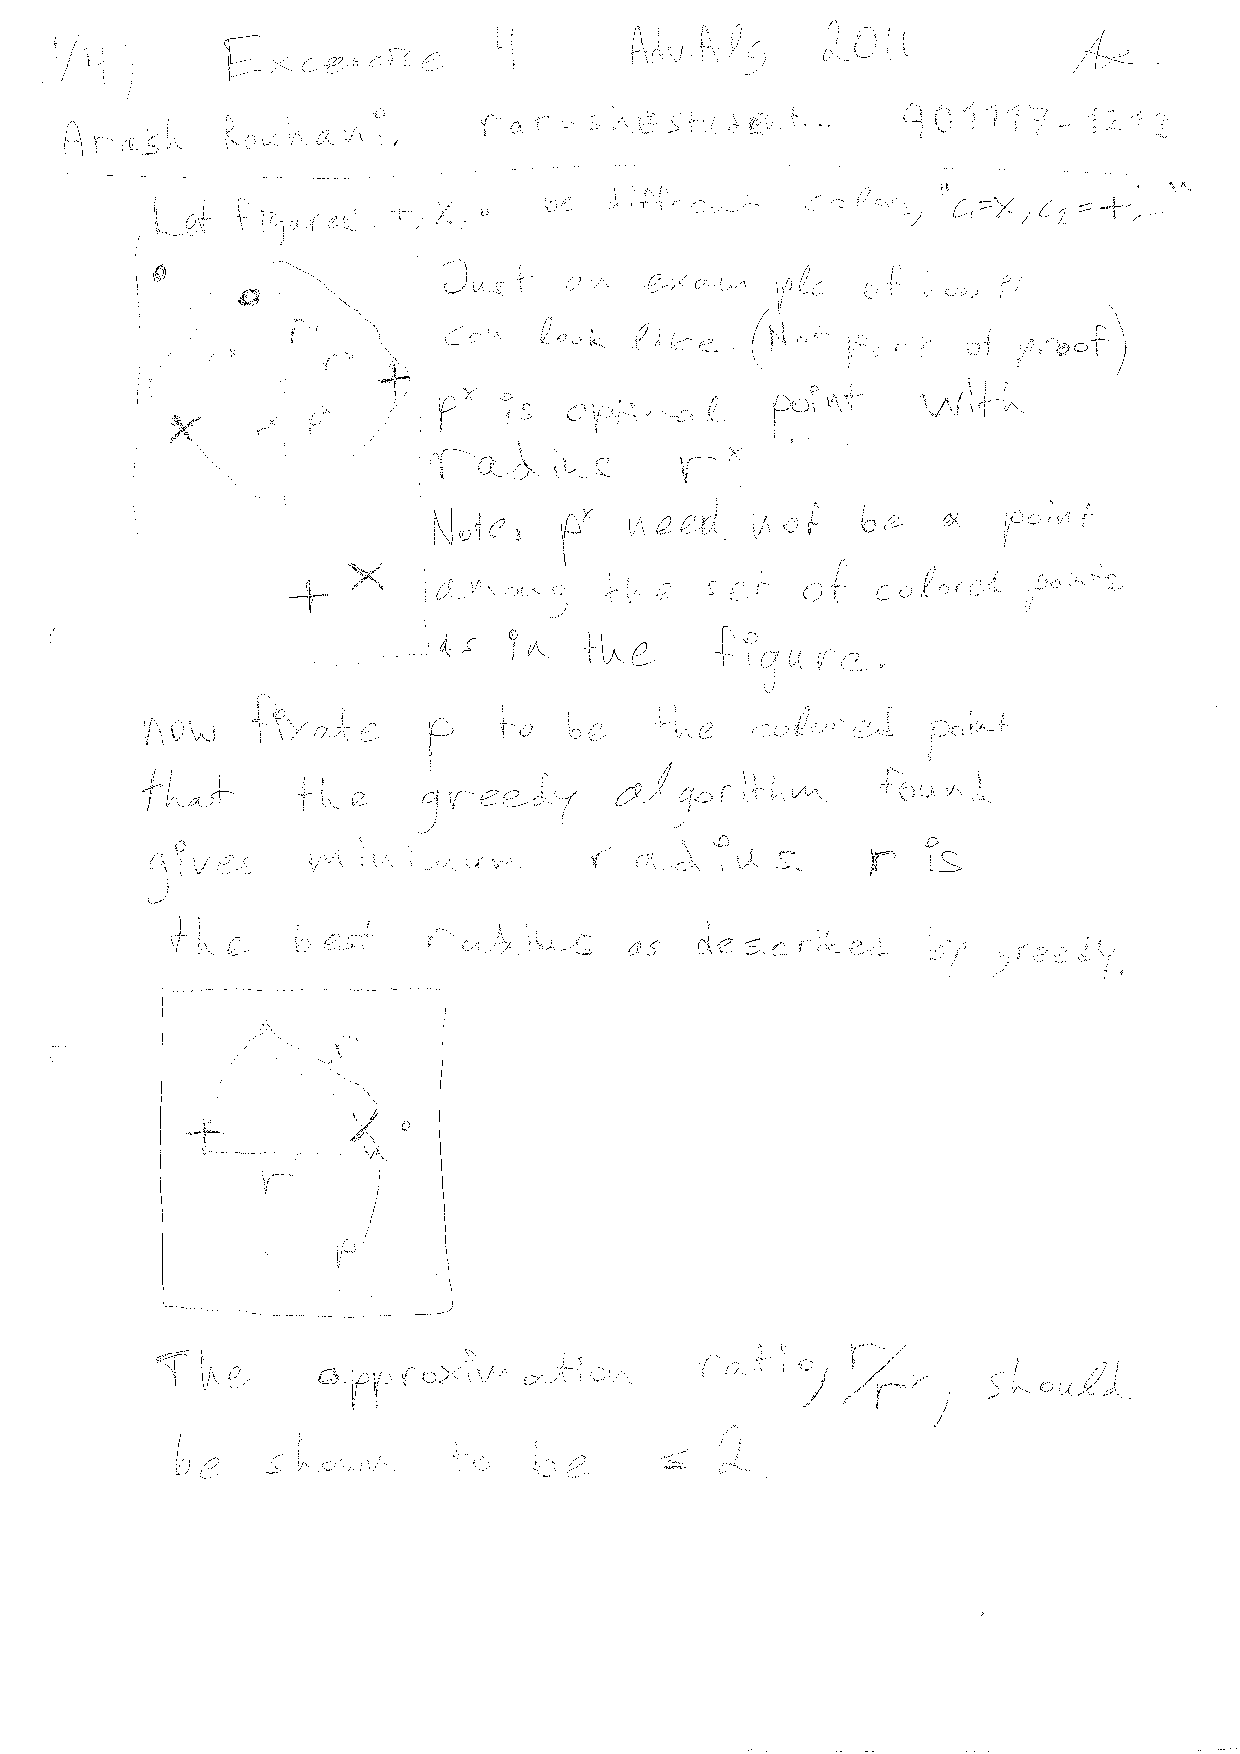
\includepdf[pages=-]{20111105191330882.pdf}

\section{Weigthed Hitting Set}

$A$ is our set with $n$ elements (our nodes), having weights $w_i$.
We have $m$ subsets $B_j$, $|B_j| \leq b$. An answer $S$ will have cost $w(S)$.
I won't repeat the whole problem formulation.

We follow the given hint, so we make an extended version of
the pricing analogy, basically, each subset pays for contained nodes.
And fair prices is held when $\forall i, \sum_{i \in B_j} p_j \leq w_i$.
So each $B_j$ has its price $p_j$.
A node is tight when $\forall i, \sum_{i \in B_j} p_j = w_i$.

\subsection{Algorithm}

Loop once over all $j$ in any order. Increase $p_j$ as much as possible
without violating fair prices (that is, until one of the nodes are tight).
The answer $S$ is the set of tight nodes.

\subsection{Analysis}

First let's assure that $S$ is a hitting set cover. $S$ must
be a solution by proof of contradiction, let's say that
the subset $B_j$ is left unhit. So will be the case if all nodes in
$B_j$ are non-tight, but that won't happen as the algorithm
was supposed to increase $p_j$ until one of the nodes in $B_j$
became tight.

By definition of the return set $S$ we have
$\forall i \in S, \sum_{i \in B_j} p_j = w_i$.
This gives $ \sum_{i \in S} \sum_{i \in B_j} p_j = w(S)$.
Every price $p_j$ will occur at most $b$ times in the sum
(exactly $b$ times if all $|B_j| = b$ and $S = A$).
So definetly $w(S) \leq b \sum_{j} p_j$.

Before drawing our last conclusion, we must note that
$\sum_{j} p_j \leq w(S) $ for \emph{any} solution $S$.
Motivation follows:
If fair prices are held, we have
$\sum_{i \in B_j} p_j \leq w_i$ and in particular
$\sum_{i \in S} \sum_{i \in B_j} p_j \leq w(S)$.
A hitting set have hitten every subset, so surely
$\sum_{j} p_j \leq \sum_{i \in S} \sum_{i \in B_j} p_j \leq w(S)$

Now we consider $S$ as the greedy solution again.
Given $w(S) \leq b \sum_{j} p_j$ and $\sum_{j} p_j \leq w(S)$.
So say the optimum weight is $K=w(S^*)$, of course
$\sum_{j} p_j \leq K \leq b \sum_{j} p_j$.
In ideal case $K = \sum_{j} p_j$,
so we conclude that our greedy won't do worse than $b$
times the optimum value. Done.

\section{Excerise 6 (showing NP-completeness)}

We will show that the problem is NP-complete:
First we show that the problem is in NP, then
we show that Set Cover reduces to our problem.

\subsection{in NP?}

We will show that given a proposed solution $F \subseteq E$
to my problem, I should be able verify that it
solves the problem (not neccesarily optimally),
that is all terminal nodes are reachable only using the $F$ edges.

\textbf{Algorithm:} Make a dfs-search from the root $r$ in the graph
$G' = (V, F)$. $F$ is a solution iff every node in $T$
was visited by the graph-search. \textbf{end.}

In general when dfs-searching from a node $s$,
the search will visit a node $t$ iff there is a path $s \to t$.
Which was what $F$ must fulfill. That is my motivation for that
the algorithm checks that $F$ is a solution.
Also, obviously it runs in polynomial time only doing a dfs.

\subsection{Reduction from Set Cover}

We will show that Set Cover ($D$) \emph{reduces to} our problem ($C$).
Here we mean the \emph{unweighted} Set Cover problem. Let the set
$A$ denote the set of choosen sets for the Set Cover problem,
then the union of all elements in $A$ is $U$.
Also all edges are two-way, that is when I write edge $(a, b)$ i mean
${a, b}$ edge.

We reduce the Set Cover instance $d = (U, S_1..S_m) \in D$ to an instance
of our problem $c = (G, T, r) \in C$. This instance to instance transformation is
already described in the problem statement and won't be repeated here.

We have the $c$ and $d$, we will show how the solutions,
$Sol_C(c) = F$ and $Sol_D(d) = A$ relate.
I claim and will motivate that $ |A| = |F| - |T| $ and
$ A = \bigcup_{(r,i) \in F} S_i$. Where we call the $S_i$'s set node
$i$. The rest of this document is to
convince that the solutions
are mapping to each-other.

An edge from an element node $x$ will only be added
to $F$ if it will be part of $x$'s path to $r$. 
Also, if we have dedicated an edge from $x$ to $i$ (denoted $x \to i$).
We will always add the edge of $i$ (= $x \to i$ ) to $F$,
as that edge leads immedietly to $r$ with only one edge.

About element nodes $x$ and set nodes $i$. Each of the $|T|$
element nodes are
responsible for adding 1 edge to one set node, since all element
nodes must "reach out" to $r$ some way.
The set nodes buy their $i \to r$ edge iff any element
bought an edge to them ($x \to i$). If I can show
that adding edge $i \to r$ corresponds to adding set $S_i$,
then clearly $|T| + |A| = |F|$.

Now think about the Set Cover problem, imagine
that any element $x$
picks which set $x \in S_i$ it is covered by, and we return
$A$ to be the union of picked sets. Now if we
imagine that these elements collaborate to pick their $S_i$
to minimize $A$. Then the set cover is optimally satisfied.
It's satisfied since every element have picked
a coverer, and optimally as $A$ is minimized.

When $x$ choose $S_i$ in Set Cover, it corresponded to
node $x$ picking edge $x \to i$ which also implied
picking $i \to r$. Running our problem will yield
$F$, and if $(r,i) \in F$ then that corresponds to
choosing set $S_i$ in the set cover.

Note that knowing optimal $F$ gives optimal $A$,
but $A$ gives only the edges of the form $(r, i) \in F$.
But the rest of the $x \to i$ edges can be trivially
assigned to first $i$ that have it's edge taken.
(such $i$ always exists)

Constructing instance $d$ from $c$ is polynomial,
and so if we can solve any $c \in C$ polynomially, we can do
for any $d \in D$ as well. We have reduced $D$ to $C$. Done.

\end{document}
